\documentclass[11pt]{article}
\usepackage[utf8]{inputenc}
\usepackage[T1]{fontenc}
\usepackage{amsmath, bm}
\usepackage{float}
\usepackage{hyperref, tikz}
\usepackage{bm}
\usepackage{tikz}
\usepackage{caption}
\usepackage{subcaption}
\usepackage{mathtools}
\usepackage{verbatim}

\usetikzlibrary{calc}
\setcounter{secnumdepth}{0}
\DeclareMathOperator{\relu}{ReLU}
\DeclareMathOperator{\sign}{sign}
\begin{document}
\begin{center}
  \mbox{}\\[2.0cm]
  \textsc{\Huge Deep Learning}\\[1.0cm]
  \textsc{\Large Homework 2}\\[0.5cm]
\end{center}
\begin{flushleft}
  Group 71 members: \\[0.5cm]
  \begin{itemize}
  \item Luis Jose De Macedo Guevara (95621)
  \item Vincent Jakl (108529)
  \end{itemize}
\end{flushleft}

\section{Contributions of each member}
\begin{itemize}
    \item Luis Jose De Macedo Guevara (95621):
    \item Vincent Jakl (108529):
\end{itemize}
\pagebreak
\section{Question 1}
\subsection{1.}
\subsection{2.}
\subsection{3.}
\subsection{4.}
\section{Question 2}
\subsection{1.}
\subsection{2.}
\subsection{3.}
\section{Question 3}
\subsection{1.}
\begin{figure}[H]
    \centering
    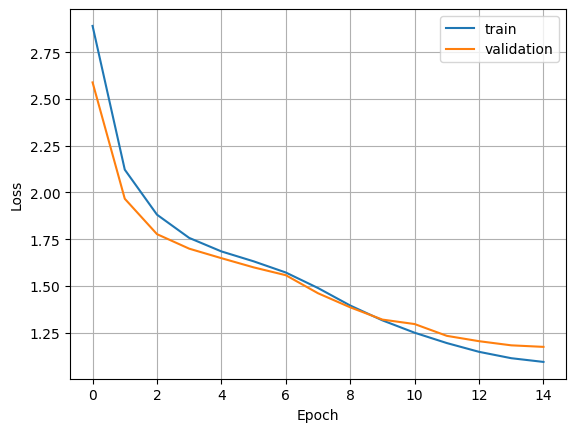
\includegraphics[width=0.8\textwidth]{./plots/recurrent_loss_per_epoch}
    \caption{Training and validation loss for the RNN model.}
    \label{fig:recurrent_loss_per_epoch}
\end{figure}

\begin{figure}[H]
\centering
\begin{subfigure}{.5\textwidth}
  \centering
  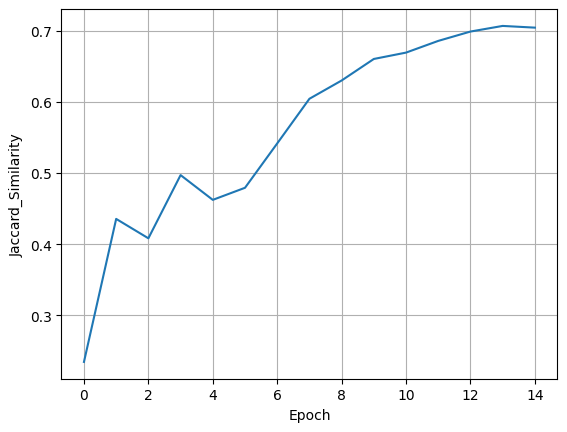
\includegraphics[width=.9\linewidth]{plots/recurrent_jaccard_similarity_per_epoch}
  \caption{Training Jaccard similarity per epoch}
\end{subfigure}%
\begin{subfigure}{.5\textwidth}
  \centering
  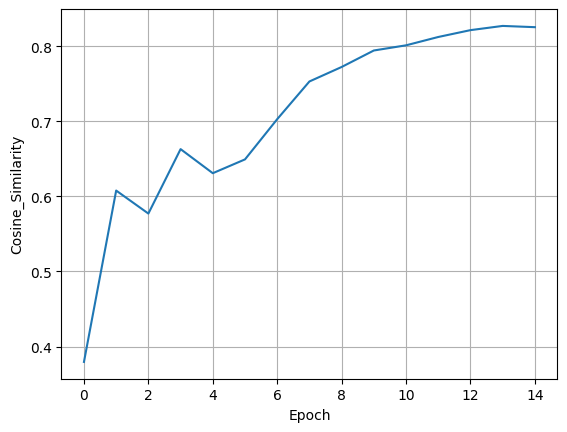
\includegraphics[width=.9\linewidth]{plots/recurrent_cosine_similarity_per_epoch}
  \caption{Training cosine similarity per epoch}
\end{subfigure}
\begin{subfigure}{.5\textwidth}
  \centering
  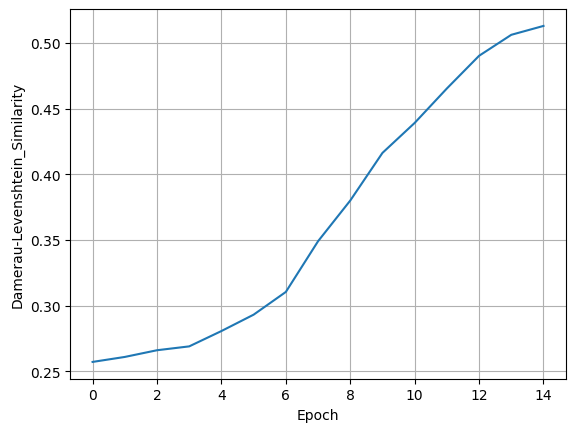
\includegraphics[width=.9\linewidth]{plots/recurrent_damerau-levenstein_similarity_per_epoch}
  \caption{Training Damerau-Levenstein similarity per epoch}
\end{subfigure}
\caption{Training similarity metrics per epoch for the RNN model.}
\label{fig:recurrent_similarity_per_epoch}
\end{figure}
The final testing metrics for the RNN were as follows:
\begin{itemize}
    \item Jaccard similarity: $0.7149$
    \item Cosine similarity: $0.8324$
    \item Damerau-Levenstein similarity: $0.5087$
    \item Loss: $1.1828$
\end{itemize}

\subsection{2.}
\begin{figure}[H]
    \centering
    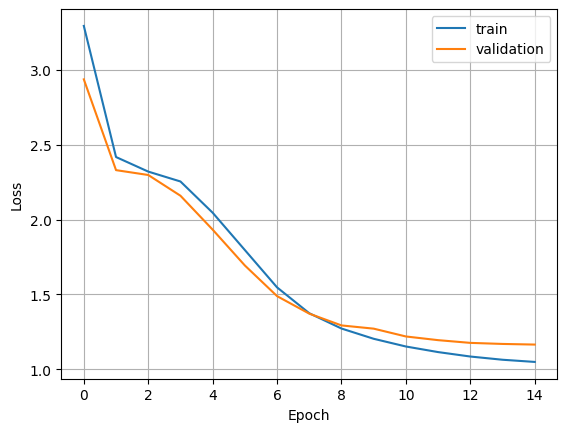
\includegraphics[width=0.8\textwidth]{./plots/transformer_loss_per_epoch}
    \caption{Training and validation loss for the RNN model.}
    \label{fig:transformer_loss_per_epoch}
\end{figure}

\begin{figure}[H]
\centering
\begin{subfigure}{.5\textwidth}
  \centering
  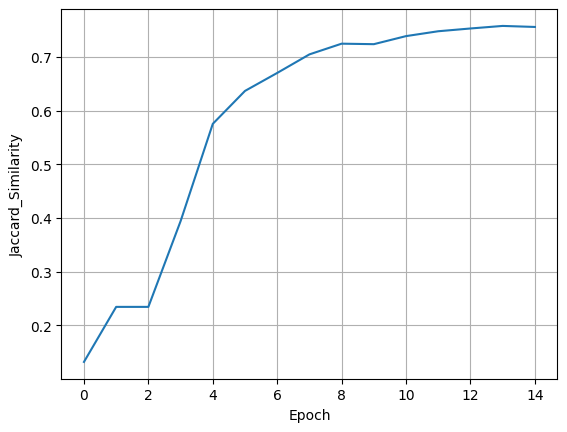
\includegraphics[width=.9\linewidth]{plots/transformer_jaccard_similarity_per_epoch}
  \caption{Training Jaccard similarity per epoch}
\end{subfigure}%
\begin{subfigure}{.5\textwidth}
  \centering
  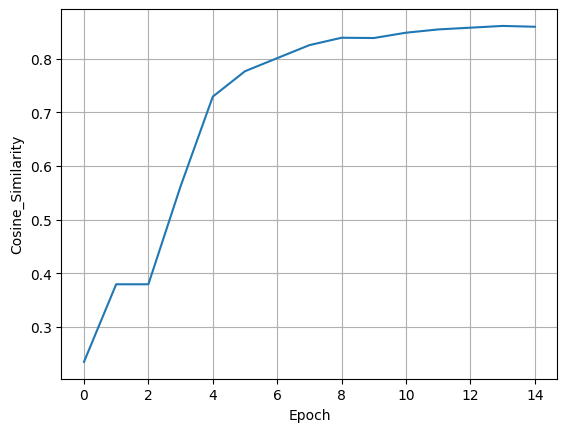
\includegraphics[width=.9\linewidth]{plots/transformer_cosine_similarity_per_epoch}
  \caption{Training cosine similarity per epoch}
\end{subfigure}
\begin{subfigure}{.5\textwidth}
  \centering
  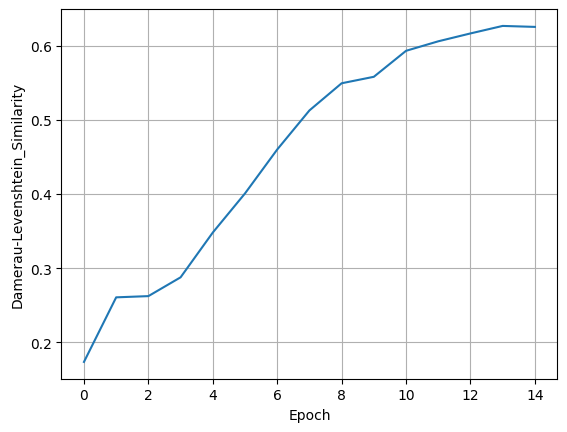
\includegraphics[width=.9\linewidth]{plots/transformer_damerau-levenstein_similarity_per_epoch}
  \caption{Training Damerau-Levenstein similarity per epoch}
\end{subfigure}
\caption{Training similarity metrics per epoch for the transformer model.}
\label{fig:transformer_similarity_per_epoch}
\end{figure}

The final testing metrics for the transformer were as follows:
\begin{itemize}
    \item Jaccard similarity: $0.7648$
    \item Cosine similarity: $0.8655$
    \item Damerau-Levenstein similarity: $0.6344$
    \item Loss: $1.1596$
\end{itemize}

\subsection{3.}
\subsection{4.}
\end{document}